\section{Métricas}
\begin{itemize}
\item Se vuelve necesario tener pautas más allá del código.
\item El 60\% de los errores es posible detectarlos tempranamente realizando revisiones de diseño tempranas.
\item ¿Qué clases revisamos? ¿Qué paquetes?
\item Esta fuertemente orientado a objetos.
\item Son medidas estáticas, para hacer un análisis estático del diseño del código escrito.
\item Si los números obtenidos (valores relativos) están dentro de los rangos esperados se esta bien, si nos desviamos hay que revisar el sistema.
\end{itemize}



\subsection*{Overview piramidal}

\begin{itemize}
\item Ubica las métricas en una pirámide
\item Cada una de estas nos van a dar conclusiones que son difíciles de sacar mirando el código, de ahí el valor de las métricas.
\end{itemize}

\begin{figure}[!htb]
    \centering
    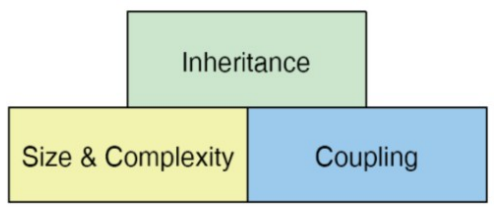
\includegraphics[width=0.6\textwidth]{img/OverviewPyramid.PNG}
\end{figure}

\subsubsection*{Tamaño y complejidad}

\begin{itemize}
\item Son proporciones calculadas
\item Permiten comparaciones independientes del tamaño de los proyectos.
\end{itemize}


\subsubsection*{Acoplamiento}

\begin{itemize}
\item Calls es el numero de invocaciones a cualquier método de una clase desde diferentes métodos de otras
\item FANOUT: nro de clases dependientes (uso, invocaciones)
\item FANOUT / CALLS: cantidad de invocaciones salientes dividida la cantidad de llamadas entrantes
\item CALLS / NOM: cantidad de llamadas entrantes dividida la cantidad de métodos
\end{itemize}

\subsubsection*{Herencia}

\begin{itemize}
\item Nos dan una idea de la profundidad o ancho de las clases.
\item ANDC: Average Number of Derived Classes. Solo se contabilizan clases (no interfaces) propias (no de librerías).
\item ANDC = sumatoria (nro clases x nro herencias por clase) / NOC
\item AHH: Average Hierarchy Height
\item AHH = sumatoria(nro clases root x nro niveles de herencia) / NOC
\end{itemize}


\begin{figure}[!htb]
    \centering
    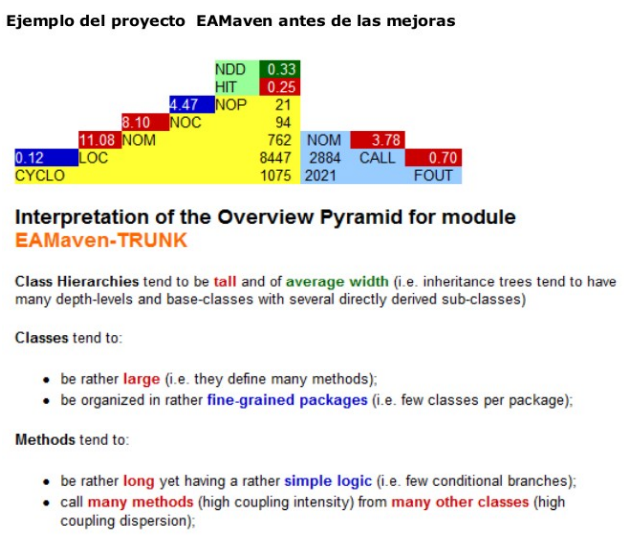
\includegraphics[width=0.8\textwidth]{img/EjemploMetricas.PNG}
    \caption{Ejemplo de la pirámide}
\end{figure}


\subsection*{Métricas y visualización estética}

\begin{itemize}
\item Se relaciona el ancho y altura de rectángulos con diferentes resultados de las métricas.
\item Se agregaron colores
\item Se agrego peso al ancho de las relaciones.
\end{itemize}

\subsubsection*{Diagrama de complejidad}

\begin{itemize}
\item Aparecen todas las clases coloreadas. Indican distintos tipos de fallas.
\end{itemize}

\begin{figure}[!htb]
    \centering
    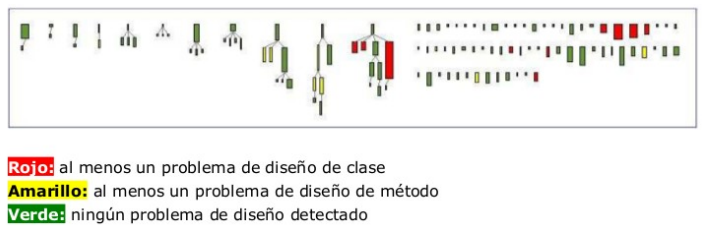
\includegraphics[width=0.8\textwidth]{img/DiagramaComplejidad.PNG}
\end{figure}

\subsubsection*{Class Blueprint}

\begin{itemize}
\item Es una representación de una clase.
\item Muestra desde el exterior al interior.
\end{itemize}

\begin{figure}[!htb]
    \centering
    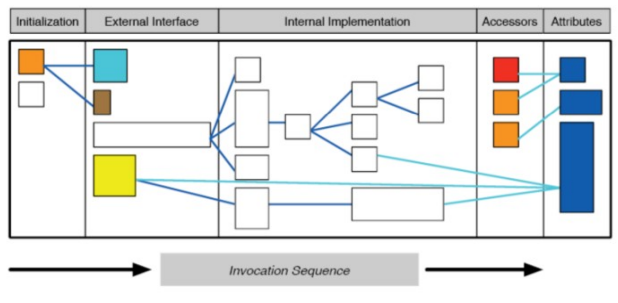
\includegraphics[width=0.8\textwidth]{img/ClassBlueprint.PNG}
\end{figure}

Los distintos colores ayudan a identificar particularidades


\subsection*{Medidas de falta de armonía}
\begin{itemize}
\item A partir de las métricas se construyo el concepto de falta de armonía
\item En amarillo de falta de identidad: Armonía entre la clase que modela un concepto y los datos y métodos que operan sobre esos datos.
\item Azul de tipo colaboración: Armonía en la forma en que colabora cada clase con el resto a efectos de lograr la funcionalidad pedida.
\item En verde de tipo clasificación: Cómo cada clase hace uso de los métodos heredados y los propios. Cuál es el comportamiento de cada clase en la jerarquía de herencia a la cual pertenece.
\end{itemize}


\begin{figure}[!htb]
    \centering
    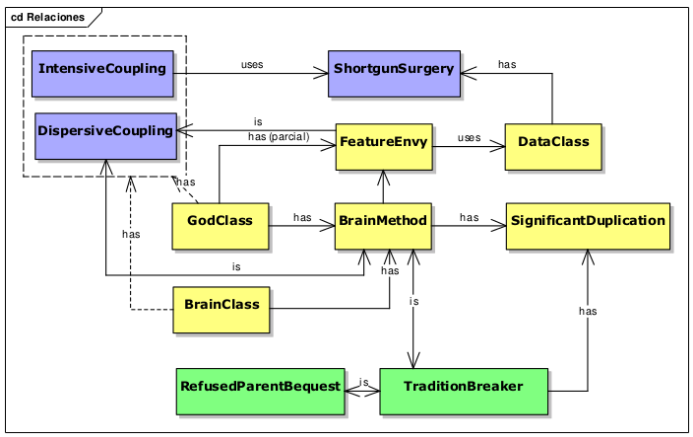
\includegraphics[width=0.8\textwidth]{img/RelacionesFaltaDeArmonia.PNG}
\end{figure}


\subsubsection*{FeatureEnvy}

\begin{itemize}
\item La presencia de una data class indica la falta de armonía de feature envy
\item Una clase esta interesada en usar atributos de otra clase
\end{itemize}

\subsubsection*{Brain Method}

\begin{itemize}
\item Método que hace todo, viola Single Responsability
\item Toma datos de lugares que no corresponde
\item El Brain Method generalmente indica la presencia de una Brain Class. Una clase que desbalancea el manejo del sistema. Que no esta claro la función que tiene.
\item También puede implicar una God Class.
\end{itemize}


\subsubsection*{Acoplamientos}
\begin{itemize}
\item Se tiene bajo acoplamiento entre clases a través de invocación de métodos con extensión (nro limitado de clases), intensidad (unidireccionales) y dispersión (mismo nivel abstracción, otro nivel, otro package) limitadas.
\item Si se tiene Excesivo funout -> muy inestable
\item Si se tiene Excesivo funin -> inmutable
\end{itemize}



\subsubsection*{Shotgun Surgery}

\begin{itemize}
\item Fuerte acoplamiento intensivo, todos los proveedores invocan un método cliente. (Singleton es un ejemplo de esto)
\end{itemize}

\subsubsection*{Transaction Factory/Registry}

\begin{itemize}
\item Muestran la dependencia entre clases
\end{itemize}


